%================================================================
\chapter{Supervised Learning}\label{chap:SupervisedLearning}
%================================================================

This chapter introduces the fundamentals of supervised learning, optimization and neural networks. The content of this chapter is mainly based on the material in \cite{SupervisedwquantumComputers}, \cite{hastie01statisticallearning} and \cite{nielsenneural}.

The goal of \emph{supervised learning}, one of the big branches of machine learning, is to obtain a function for predicting an output $y$ from an input $\boldsymbol{x}$. This is done by learning from input-output pairs $\mathcal{T} = \{(\boldsymbol{x}^{(1)}, y^{(1)}), \cdots, (\boldsymbol{x}^{(N)}, y^{(N)})\}$, known as the training set. The domain of the input and output depends on the specific learning problem. The output y, also called the target or the response, is often either of a quantitative or qualitative character. These two cases constitutes two big paradigms in supervised learning: \emph{regression} and \emph{classification}, respectively. In the case of regression, the goal of the learning task is to predict a real-valued target y from the input $\boldsymbol{x}$. Typical examples of targets to regress on are \emph{temperature}, \emph{weight} and \emph{number of people}, which have in common a natural notion of distance measure in the sense that instances close in numerical value are also close in nature. E.g., two fish weighing $12.1$ kg and $12.2$ kg are similar, while a third fish weighing $24.0$kg is notably different.

For classification, the goal is to predict one or more \emph{classes} from an input $\boldsymbol{x}$. In this setting, the target $y$ is discrete and categorical, such as \emph{color}, \emph{dead/alive} and \emph{type of animal}. In contrast to quantitative targets, qualitative targets lack a natural distance measure, in the sense that it is not meaningful to compare the distance between \emph{dog} and \emph{cat}, and \emph{dog} and \emph{seagull}. They are simply mutually exclusive classes.

The input $\boldsymbol{x}$ is a vector consisting of elements $(x_1, \cdots, x_p)$ often called features and predictors. Each feature $x_i$ can either be quantitative or qualitative in the same manner as with the target previously discussed. In this thesis, we will be investigating quantitative features $\boldsymbol{x} \in \mathbb{R}^{p}$.


%================================================================
\section{Parametric Models}\label{sec:ParametricModels}
%================================================================
The approach of supervised learning often starts by acquiring a training set $\mathcal{T} = \{(\boldsymbol{x}^{(1)}, y^{(1)}), \cdots, (\boldsymbol{x}^{(N)}, y^{(N)})\}$, where $N$ is the number of samples in the training set. This is called labeled data, since the samples of features $\boldsymbol{x}^{(i)}$ are accompanied by the ground truth target $y^{(i)}$(the labels of the samples) that we would like to predict. One often hypothesises that the acquired training data was produced by some mechanism or process that we can mathematically express as

\begin{equation*}
    y = f(\boldsymbol{x}) + \epsilon,
\end{equation*}
where $\epsilon$ is often included to account for randomness, noise or errors in the data, in contrast to the deterministic part $f(\boldsymbol{x})$. Depending on the context, the $\epsilon$ may be neglected or assumed to be normally distributed such as $\epsilon \sim \mathcal{N}(0, \sigma^2)$, where $\sigma^2$ is the variance.

The goal is to approximate the underlying mechanism $f(\boldsymbol{x})$. To do this, one often proposes a parametric model

\begin{equation*}
    \hat{y} = f(\boldsymbol{x}; \boldsymbol{\theta}),
\end{equation*}

where $\hat{y}$ is the predicted value, $f(\cdot; \cdot)$ defines a \emph{family} of models, and $\boldsymbol{\theta}$ is a specific vector of parameters that defines a specific model from the this family. Training the model on involves finding the parameters $\boldsymbol{\theta}$ such that the model best reproduces the target from the features found in the training data set. To quantify what is meant by "best" in this context, it is common to introduce a \emph{loss function} that measures the quality of the model with respect to the training data set:

\begin{equation}\label{eq:LossFunction}
    L(\boldsymbol{\theta}) = \frac{1}{N}\sum_{i=1}^{N} L(f(\boldsymbol{x}^{(i)}; \boldsymbol{\theta}) , y^{(i)}),
\end{equation}

The loss function returns a scalar value that measures how good your model fits the training data for a particular set of parameters. In general, a smaller value indicates a better model. This formulates the task of training the model as an optimization problem. In the next section, we will discuss different ways of training parameterized models, in particular with the use gradient-based methods.

The choice of loss function is very problem dependent, and there is a vast collection of different choices in the machine learning literature. In this thesis we will focus the popular Mean Squared Error(MSE) when training supervised learning models. This loss function is suitable for regression problems since it implements a natural distance measure between prediction and target. It is formulated as

\begin{equation}\label{eq:MSE}
    MSE = \frac{1}{2N}\sum_{i=1}^{N} (f(\boldsymbol{x}^{(i)}; \boldsymbol{\theta}) - y^{(i)})^2.
\end{equation}

Fitting the model using MSE as loss function is often referred to as \emph{least squares approach}.




%================================================================
\section{Optimization}\label{sec:Optimization}
%================================================================
Finding the optimal parameters $\hat{\boldsymbol{\theta}}$ with respect to a chosen loss function $L$ can be formulated as

\begin{equation}\label{eq:Optimization}
    \hat{\boldsymbol{\theta}} = \underset{\boldsymbol{\theta}}{\argmin} \frac{1}{N}\sum_{i=1}^{N} L(f(\boldsymbol{x}^{(i)}; \boldsymbol{\theta}) , y^{(i)}).
\end{equation}

This optimisation problem is not in general easy, and depends highly on the choice of loss function and parametric model. Aside from a few exceptions, like the case of linear regression, \autoref{eq:Optimization} does not generally have an analytical solution. More over, many popular parametric models results in non-convex optimisation problems, meaning the \emph{loss landscape} exhibit several local minima. In practice, such optimization problems can't be solved efficiently(STEPHEN A. VAVASIS). However, it is important to realize that an exact, or close to exact, minimization of the loss function is seldom needed or even favourable. What is ultimately interesting is whether the trained model has sufficient ability to predict. Over the years, several cheap and approximate methods for optimization have been invented to train machine learning models. We will discuss two such methods that implement gradient-based optimization. 

%================================================================
%\subsection{Matrix Inversion}\label{sec:MatrixInvertion}
%================================================================
%(uferdig avsnitt, skal kanskje droppes)
%Linear regression models are defined as 

%\begin{equation*}
%    f(\boldsymbol{x}; \boldsymbol{\beta}) = \sum_{j=0}^p x_j \beta_j =  \boldsymbol{x}^T %\boldsymbol{\beta},
%\end{equation*}
%where $\boldsymbol{x}^T = [1, x_1, \cdots, x_p]$ is a vector of $p$ features together with a constant $1$ %to account for the intercept of the model, and $\boldsymbol{\beta}$ is a vector of model parameters %called coefficients. Using least squares approach leads to the following loss function:

%\begin{equation*}
%    L(\boldsymbol{\theta}) = \frac{1}{N}\sum_{i=1}^{N} (\sum_{j=0}^p x_j^{(i)} \beta_j -  y^{(i)})^2.
%\end{equation*}

%This objective function can be reformulated using matrix and vector notation as

%\begin{equation*}
%    L(\boldsymbol{\theta}) = (\boldsymbol{X}\boldsymbol{\beta} - %\boldsymbol{Y})^T(\boldsymbol{X}\boldsymbol{\beta} - \boldsymbol{Y}),
%\end{equation*}
%where $\boldsymbol{X}^T = [\boldsymbol{x^}]$ 

%================================================================
\subsection{Batch Gradient Descent}\label{sec:GradientDescent}
%================================================================
In the absence of an analytical expression that minimizes the loss function, \emph{gradient descent} is an easy-to-implement method that iterativly decreases the loss. This is done by repeatedly adjusting the model parameters using information of the \emph{gradient} of the loss function. The derivative of the loss function with respect to the model parameters can be calculated as

\begin{equation}\label{eq:LossDerivateWRTparameter}
    \frac{\partial}{\partial \boldsymbol{\theta}_k} L(\boldsymbol{\theta}) =
    \frac{1}{N}\sum_{i=1}^{N} \frac{\partial}{\partial \hat{y}^{(i)}} L( \hat{y}^{(i)}, y^{(i)})
    \frac{\partial}{\partial \boldsymbol{\theta}_k}\hat{y}^{(i)}
\end{equation}
where $\boldsymbol{\theta}_k$ is the k'th model parameter, and  $\hat{y}^{(i)} = f(\boldsymbol{x}^{(i)}; \boldsymbol{\theta})$. To arrive at this expression, the chain rule was used under the assumption the the loss function $L(\hat{y}^{(i)}, y^{(i)})$ and model output $\hat{y}^{(i)}$ are differentiable with respect to $\hat{y}^{(i)}$ and $\boldsymbol{\theta}_k$, respectively. Notice that the derivative is calculated with respect to the entire training set, i.e. the whole \emph{batch}, hence the name. The gradient is then constructed simply as a vector quantity containing the derivatives with respect to each model parameter:

\begin{equation}\label{eq:Gradient}
    \nabla_{\boldsymbol{\theta}} L(\boldsymbol{\theta})= 
    \big{(} \frac{\partial}{\partial \boldsymbol{\theta}_1} L(\boldsymbol{\theta}), 
    \cdots, \frac{\partial}{\partial \boldsymbol{\theta}_p} L(\boldsymbol{\theta}) \big{)}
\end{equation}

The gradient \autoref{eq:Gradient} can be geometrically interpreted as  the direction at point $\boldsymbol{\theta}$ in parameters space for which the value of the loss function increases most rapidly(kilde). In light of this, one can attempt to move all the parameters some small amount in the opposite direction, \emph{the direction of steepest descent}, in order to decrease the loss. This can be done recursively, and can be formulated as 


\begin{equation}\label{eq:ParameterUpdate}
    \boldsymbol{\theta}_{t} = \boldsymbol{\theta}_{t-1} - \mu \nabla_{\boldsymbol{\theta}} L(\boldsymbol{\theta}_{t-1})
\end{equation}
for $t=0, \cdots, T-1$. Here, $T$ is the total number of iterations, and $\mu$ is some small positive value, often called the \emph{learning rate}. Usually, some initial choice of parameters $\boldsymbol{\theta}_{0}$ is chosen in a random fashion. The proceeding recalculation of the gradient and repeated adjustment of the parameters results in a gradual descent in the the loss landscape, analogous to walking down a mountain. This is the heart of gradient descent.

Even though batch gradient descent is intuitively simple and sometimes sufficiently effective for training some models, it has several flaws that should be addressed when suggesting better methods of optimization. A common problem with batch gradient descent is that optimisation can have a tendency of getting stuck in local minima, as only local information in the loss landscape is used when updating the parameters. In addition, the presence of \emph{plateaus}, areas of particular flatness in the loss landscape, tend to induce slow convergence. The two aforementioned phenomena is illustrated in figure(to come). Further more, the presence of high degree of distortions in certain directions in parameter space, so called  \emph{thin valleys}, can lead to oscillations and inefficient optimization. This is exemplified in figure(). We will discuss how the particularly popular \emph{Adam optimizer}, which was used in this thesis, addresses these problems. 


\begin{figure}[htp]
    \centering
    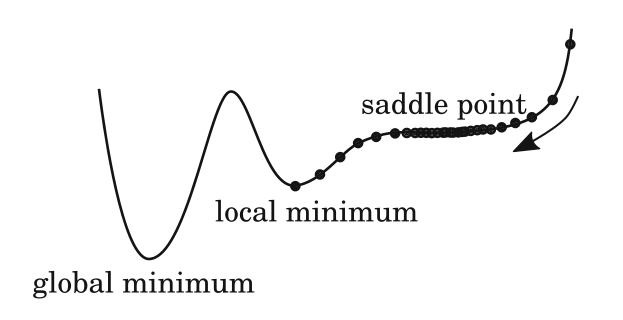
\includegraphics[width=10cm]{latex/figures/local_minimum_saddle_point.png}
    \caption{One-dimensional representation of the loss landscape for a parameterized model, showcasing the phenomenon of getting stuck in local minima, and slow convergence induced by plateaus. The figure is retrieved from (hands-on ML).}
    \label{fig:localMinima}
\end{figure}

\begin{figure}[htp]
    \centering
    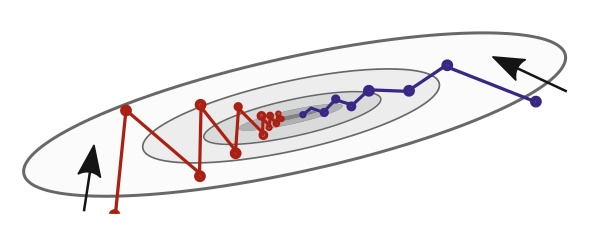
\includegraphics[width=8cm]{latex/figures/thin_vally.png}
    \caption{Two-dimensinal representation of the loss landscape for a parameterized model, illustrating a thin valley. The optimization steps in red showcase optimization without momentum. Optimization steps in blue implements momentum, showing dampened oscillation and better convergence. The figure is retrieved from (SLwQH)}
    \label{fig:thinValley}
\end{figure}

%================================================================
\subsection{Adam Optimizer}\label{sec:AdamOptimizer}
%================================================================
Introduced by (kilde), the Adam algorithm implements a moving average of the gradient, called \emph{momentum}, together with a rescaling. Replacing \autoref{eq:Gradient} and \autoref{eq:ParameterUpdate}, Adam implements the following algorithm:

\begin{algorithm}[H]\label{alg:Adam}
\SetAlgoLined

$m_0 \gets 0$;\\
$v_0 \gets 0$;\\
$t \gets 0$;\\
\While{$\theta_t$ not converged}{
t \gets t+1\\
$g_t \gets \nabla_{\theta} L(\theta_{t-1})$
(Get gradients w.r.t. loss at timestep t)\\
$m_t \gets \beta_1 m_{t-1} + (1-\beta_1) g_{t}$
(Update biased first moment estimate)\\
$v_t \gets \beta_2 v_{t-1} + (1-\beta_2) g_{t}^2$
(Update biased second raw moment estimate)\\
$\hat{m}_t \gets m_t/(1 - \beta_1^{t})$
(Compute bias-corrected first moment estimate)\\
$\hat{v}_t \gets v_t/(1 - \beta_2^{t})$
(Compute bias-corrected second raw moment estimate)\\
$\theta_t \gets \theta_{t-1} - \alpha \hat{m}_t/(\sqrt{\hat{v}_t} + \epsilon)$
(Update parameters)\\
}
\Return{$\theta_t$}
\caption{\emph{Adam}, (kilde). The authors suggest default hyperparameters $\alpha = 0.001$, $\beta_1 = 0.9$, $\beta_2 = 0.999$ and $\epsilon = 10^{-8}$. The algorithm is applied parameter-wise.}
\end{algorithm}

\autoref{alg:Adam} updates moving averages of the gradient $m_t$ and its square $v_t$, picking up information about the gradient from earlier update events. In particular, if the gradient tend to flip sign for certain directions, the averaging over previous iterations tends to dampen these oscillations. Likewise, directions of persistent sign tends to accumulate magnitude, making the optimisation gain "momentum" in these directions. This is a good property for overcoming thin valleys and plateaus. Also, the effect of momentum may also help avoid getting stuck in local minima by gracing over them. Further, the moving average of the gradient and its square is made unbiased as $\hat{m}_t = m_t/(1-\beta_1)$ and $\hat{v}_t = v_t/(1-\beta_2)$. Since the averages are initialized as zero, it is biased downward. Finally, the parameters are shifted by the quantity $\alpha \frac{\hat{m}_t}{\sqrt{\hat{v}_t} + \epsilon}$. Here, the rescaling term $\sqrt{\hat{v}_t}$ serves to decrease the step size in directions where the gradient has a large magnitude and increase it where it is small. This effectively implements a variable learning rate for each direction, depending on whether big or small steps are needed. 

Adam is a hugely successful algorithm for optimizing machine learning models, and it is praised for its robustness. The default hyper parameters are often sufficient to obtain good results. Further, the authors point out that Adam is suited for very noisy gradients, which will be relevant for the work in this thesis. 



%================================================================
\section{Dense Neural Network}\label{sec:DenseNeuralNetwork}
%================================================================
Originally inspired by the network structure of the brain(kilde), artificial neural networks are powerful parameterized machine learning models that have proved to extremely useful for a vast number of applications. Over the years, a comprehensive collection of different network architectures have been developed to target specific problems, such as \emph{Recurrent Neural Networks} for predicting time series data and \emph{Convolutional Neural Networks} for image classification. In this thesis, we will focus on \emph{Dense Neural Networks}, which is a simple \emph{feedforward network}, meaning the information is processed in a forward fashion without any loops.

%================================================================
\subsection{Feedforward}\label{sec:FeedforwardDNN}
%================================================================
Dense Neural Networks works by sequentially transforming input data by passing them through one or more \emph{layers}, which each applies a paramaterized and often non-linear transformation. The result of the first layer of the neural network can be formulated as

\begin{equation}\label{eq:FeedforwardSingle}
    \boldsymbol{a}^1 = f^1(\boldsymbol{z}^1) = f^1(W^1 \boldsymbol{x} + \boldsymbol{b}^1),
\end{equation}
Here, $\boldsymbol{x} \in \mathbb{R}^p$ is a single sample of $p$ features. $W^1 \in \mathbb{R}^{m \times p}$ and $\boldsymbol{b}^1 \in \mathbb{R}^{m}$ are a matrix and a vector of parameters called the \emph{weights} and \emph{biases}, respectively. The operations $W^1 \boldsymbol{x} + \boldsymbol{b}^1$ applies an affine transformation of the features resulting in $m$ new derived features, each identified as a \emph{node} in the specific layer. Further, $f^1(\cdot)$ is a layer-specific function, often monotonous and non-linear, applied element-wise on the derived features. This finally results in the output of the layer, $\boldsymbol{a}^1$, called the \emph{activation}.

We will now generalize \autoref{eq:FeedforwardSingle} to an arbitrary layer. For a neural network with $L$ layers, the feedforward procedure for layer $l$  can be formulated as 

\begin{equation}\label{eq:FeedforwardDNN}
    \boldsymbol{a}^l = f^l(\boldsymbol{z}^l) = f^1(W^l \boldsymbol{a^{l-1}} + \boldsymbol{b}^l),
\end{equation}
where $\boldsymbol{a}^{l-1}$ is the activtion of the previous layer with the exception $\boldsymbol{a}^{0} = \boldsymbol{x}$. The output of the network is then the activation of the last layer, namely 
\begin{equation}\label{eq:neuralNetwork}
    \hat{y} = f(x;\boldsymbol{\theta}) = \boldsymbol{a}^{L},
\end{equation}
where $\boldsymbol{\theta} = [W^1, \boldsymbol{b}^1, \cdots, W^L,  \boldsymbol{b}^L]$. This defines the whole forward procedure of a neural network, and also highlights the role of the functions $f^l(\cdot)$, often called the \emph{non-linearities}. If set to identity, $f^l(x) = x$, the recursive application of \autoref{eq:FeedforwardDNN} would simply apply repeated affine transformations, which is just an affine transformation in itself. In other words, increasing the number of layers would not increase the expressiveness of the network, as all the layers would collapse into a single layer. Therefore, introducing non-linear transformations is necessary to increase the flexibility of the neural network(kilde). 

%================================================================
\subsection{Backpropagation}\label{sec:BackpropogationDNN}
%================================================================

Neural network are typically trained using gradient-based methods, such as Batch Gradient Descent and Adam previously discussed. Adam is particularly efficient, as the optimisation of neural network architectures tend to be plagued by many local minima and plateaus(kilde).  

Assume that $f(\boldsymbol{x}^{(i)}; \boldsymbol{\theta})$ is a dense neural network as described by \autoref{eq:FeedforwardDNN} and \autoref{eq:neuralNetwork}. In order to use gradient-based methods, one needs to calculate the derivative of the loss-function \autoref{eq:LossDerivateWRTparameter} for an arbitrary parameter $\boldsymbol{\theta}_k$, which could be any of the weights $W^l$ or biases $\boldsymbol{b}^l$ in the various layers. This is not trivial given the sequential structure of the neural network. Often attributed to (kilde), the \emph{backpropagation algorithm} calculates the gradient in a sequential manner, starting with the last layers first. Calculating on a single sample, the algorithm starts by calculating the \emph{error} of the last layer


\begin{equation}\label{eq:lastLayerError}
    \delta^L_k = \frac{\partial L(\hat{y}, y)}{\partial \boldsymbol{a}^L_k},
\end{equation}
where $k$ indicates the node.

This error can be defined for any layer recursively by repeated application of the chain-rule:
\begin{equation}\label{eq:error}
    \delta^l_j = \frac{\partial L(\hat{y}, y)}{\partial \boldsymbol{a}^l_j} 
    = \sum_k \frac{\partial L(\hat{y}, y)}{\partial \boldsymbol{a}^{l+1}_k} \frac{\partial \boldsymbol{a}^{l+1}_k}{\partial \boldsymbol{a}^{l}_j}
    = \sum_k \delta^{l+1}_j \frac{\partial \boldsymbol{a}^{l+1}_k}{\partial \boldsymbol{a}^{l}_j}.
\end{equation}
This relation is the origin of the name \emph{backpropogation}, as the error terms $\delta^l$ "propagate" backwards through the neural network as they are calculated.

Using that 
$\frac{\partial \boldsymbol{a}^{l}_k}{\partial W^l_{ij}} = f^l'(\boldsymbol{z}^{l}_k)\boldsymbol{a}^{l-1}_j I_{ik}$ 
and 
$\frac{\partial \boldsymbol{a}^{l}_k}{\partial \boldsymbol{b}^l_{i}} = f^l'(\boldsymbol{z}^{l}_k) I_{ik}$, the derivative with respect to the weights and biases can then be calculated as 

\begin{equation}\label{eq:derivweights}
    \frac{\partial L(\hat{y}, y)}{\partial W^l_{ij}} = 
    \sum_k \frac{\partial L(\hat{y}, y)}{\partial \boldsymbol{a}^{l}_k} \frac{\partial \boldsymbol{a}^{l}_k}{\partial W^l_{ij}} = 
    \sum_k \delta^{l}_k f^l'(\boldsymbol{z}^{l}_k)\boldsymbol{a}^{l-1}_j I_{ik}=
    \delta^{l}_i f^l'(\boldsymbol{z}^l_i) \boldsymbol{a}^{l-1}_j,
\end{equation}
and
\begin{equation}\label{eq:derivbiases}
    \frac{\partial L(\hat{y}, y)}{\partial \boldsymbol{b}^l_{i}} = 
    \sum_k \frac{\partial L(\hat{y}, y)}{\partial \boldsymbol{a}^{l}_k} \frac{\partial \boldsymbol{a}^{l}_k}{\partial \boldsymbol{b}^l_{i}} = 
    \sum_k \delta^{l}_k f^l'(\boldsymbol{z}^{l}_k)\boldsymbol{a}^{l-1}_j I_{ik}=
    \delta^{l}_i f^l'(\boldsymbol{z}^l_i).
\end{equation}

The final gradient, over all samples, is then the average of all the single-sample gradients

\begin{equation}\label{eq:derivbiases}
    \nabla_\theta L(\theta) = \frac{1}{N}\sum_{i=1}^N \nabla_\theta L(\hat{y}^{(i)}, y^{(i)}),
\end{equation}
which can be used to optimize the neural network with a gradient-based method as discussed earlier.

\subsubsection{Universality of Dense Neural Networks}